\documentclass[a4paper]{article}
\usepackage{graphicx}
\usepackage{amsmath,amssymb,amstext}
\usepackage{graphicx}

\begin{document}

\subsubsection{CompareChildrenEqualType}

  \begin{description}
  \item[testcase\_01]  Alle 3 Kinder haben den selben Typ.
    
   \begin{equation*}
   Similarity = \frac{1+1+1}{3}=1
   \end{equation*}
    
	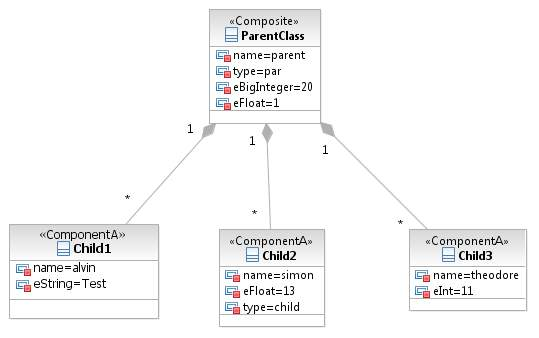
\includegraphics[scale=0.5]{CompareChildrenEqualTypeTestScreens/Testcase01model1.jpeg}
	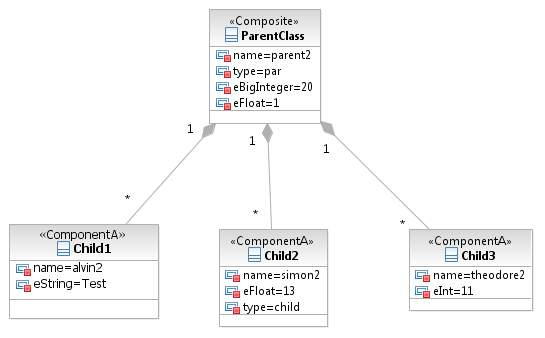
\includegraphics[scale=0.5]{CompareChildrenEqualTypeTestScreens/Testcase01model2.jpeg}

  \item[testcase\_02] 2 von 3 Kindern haben den gleichen Typ.
    
   \begin{equation*}
   Similarity = \frac{1+1+0}{3}=\frac{2}{3}
   \end{equation*}
    
	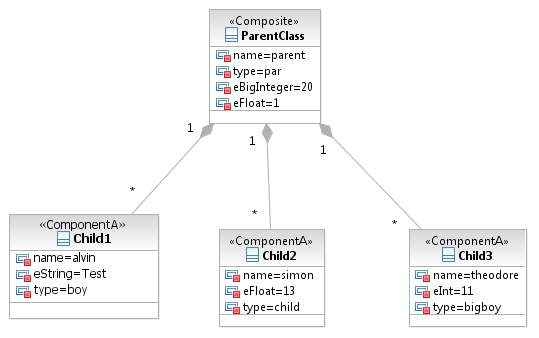
\includegraphics[scale=0.5]{CompareChildrenEqualTypeTestScreens/Testcase02model1.jpeg}
	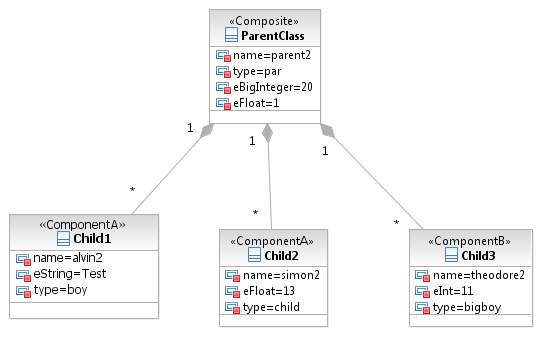
\includegraphics[scale=0.5]{CompareChildrenEqualTypeTestScreens/Testcase02model2.jpeg}

  \item[testcase\_03] Modell 1 hat 2 Kinder Typ A und 1 Kind Typ B. Modell 2 umgekehrt.
  
   \begin{equation*}
   Similarity = \frac{0+1+0}{3}=\frac{1}{3}
   \end{equation*}
    
	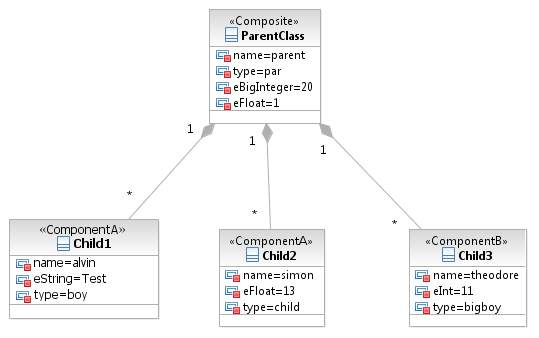
\includegraphics[scale=0.5]{CompareChildrenEqualTypeTestScreens/Testcase03model1.jpeg}
	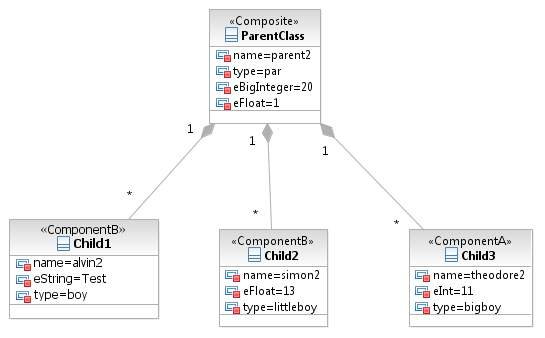
\includegraphics[scale=0.5]{CompareChildrenEqualTypeTestScreens/Testcase03model2.jpeg}

  \item[testcase\_04] Es werden 2 Modelle verglichen, wo die Klassen gleich sind, sich jedoch die Anzahl der Kinder unterscheidet.
  
   \begin{equation*}
   Similarity = \frac{1+0+1}{3}=\frac{2}{3}
   \end{equation*}
    
	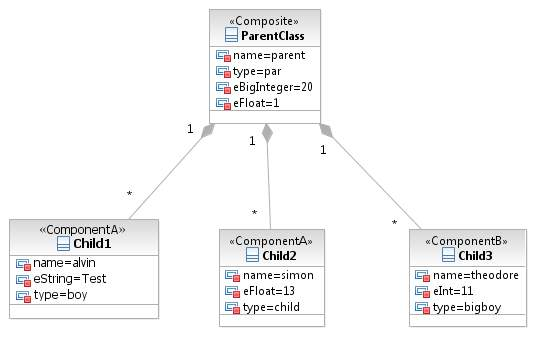
\includegraphics[scale=0.5]{CompareChildrenEqualTypeTestScreens/Testcase04model1.jpeg}
	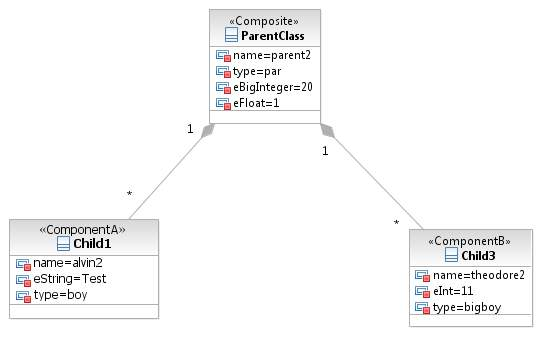
\includegraphics[scale=0.5]{CompareChildrenEqualTypeTestScreens/Testcase04model2.jpeg}
	\end{description}



\end{document}